\documentclass[a4paper,12pt,obeyspaces,spaces,hyphens]{article}
\usepackage[utf8]{inputenc}
\usepackage[T1]{fontenc}
\usepackage[normalem]{ulem}
\usepackage[vmargin=2cm, hmargin=1.5cm]{geometry}
\usepackage{fancyhdr}      % Used for customization of header/foter
\pagestyle{fancy}
\usepackage{graphicx}
\usepackage{titlesec}      % Used for \titleformat
\usepackage[htt]{hyphenat} % I want hyphenation in {\tt ...} blocks
\usepackage{xcolor}
\usepackage{titling}
\usepackage{eurosym}
\usepackage{ifthen}
\usepackage{hyperref}
\usepackage[all]{hypcap}
\usepackage{xparse}

\usepackage[most]{tcolorbox}
\definecolor{bg}{RGB}{220,220,220}

% A nicer font
\usepackage{palatino}

%% Remove indentation on the first line of each paragraph, and add
%% some space between each paragraph.
\usepackage{parskip}

\hypersetup{colorlinks=true,linkcolor=gray,urlcolor=gray}

\fancyhead{}
\fancyfoot{}

\fancyhead[CO, CE]{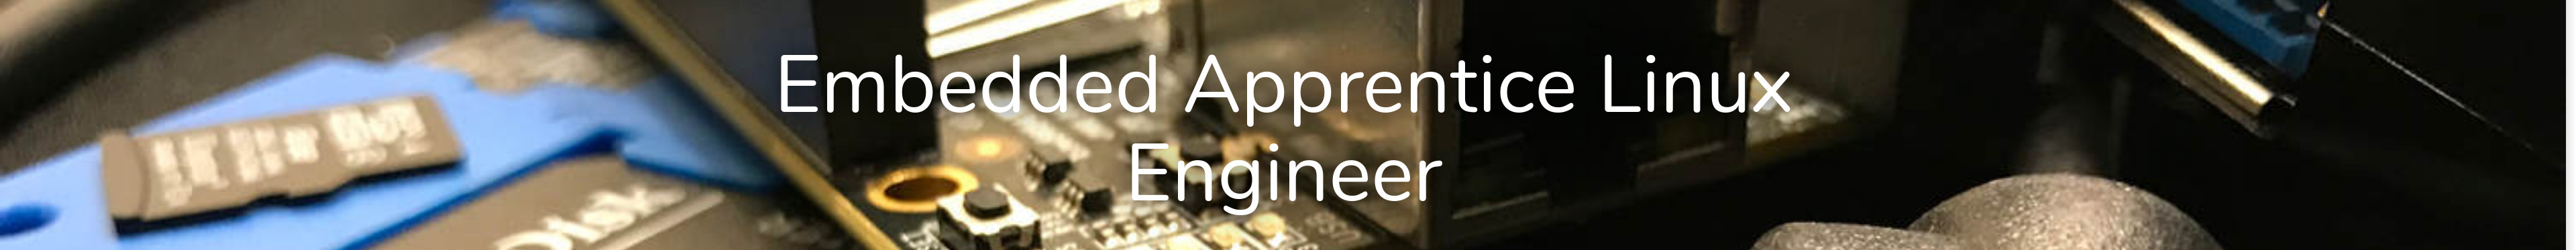
\includegraphics[width=\textwidth]{header.jpg}}
\fancyfoot[RO, LE] {\thepage}
\fancyfoot[LO, RE] {\small Embedded Apprentice Linux Engineer - Getting started with Buildroot - \url{https://www.toganlabs.com}}

\renewcommand{\headrulewidth}{0pt}
\renewcommand{\footrulewidth}{0.5pt}

\setlength{\textheight}{56em}

\definecolor{textcolor}{HTML}{4B6FA9}

% Header style
\titleformat{\section}{\color{textcolor}\normalfont\Large\sffamily\bfseries}{}{1em}{}[\vspace{2pt}\titlerule]
\titleformat{\subsection}[display]{\normalfont\large\sffamily}{}{0pt}{}[\vspace{2pt}\titlerule]
\titleformat{\subsubsection}[display]{\normalfont\sffamily}{}{0pt}{}

% No section numbering
\setcounter{secnumdepth}{0}

% Customization of title and author style
\pretitle{\begin{center}\Huge\sffamily}
\preauthor{\begin{center}
\large \sffamily \lineskip 0.2em%
\begin{tabular}[t]{c}}
\postauthor{\end{tabular}\par\end{center}}
\predate{\begin{center}\large\sffamily}

% Useful definitions

\newcommand{\code}[1]
{\path{#1}}

\hypersetup{pdftitle={Getting started with Buildroot - Lab},
  pdfauthor={Trevor Woerner, Togán Labs}}

\title{Getting started with Buildroot - Lab}
\author{Trevor Woerner, Togán Labs}

\begin{document}

\maketitle
\thispagestyle{fancy}

These lab instructions are written for the {\em Getting started with
  Buildroot} tutorial of the {\em Embedded Apprentice Linux Engineer}
track. They are designed to work for the {\em PocketBeagle} hardware
platform.

This lab is broken out into two separate paths:
\begin{itemize}
  \item Basic Lab
  \item In-Depth Lab
\end{itemize}

Both labs start with the same resources, and both end up creating the same
artifacts, but they both take different routes. If you would like to get
an image up-and-running on your board without worrying too much about the
details, take a look at the {\bf Basic Lab}. If you'd like to know a little
more about what's going on "under the hood", try the {\bf In-Depth Lab}.

Both labs start with the same {\bf Initial Setup}.

All the work for these labs occur on the {\bf host} computer, not the target.
A reasonably recent Linux machine/VM is required for this work.

\section{Initial Setup}

Our first step is to obtain the buildroot meta-data. Normally this would be
done by simply cloning from buildroot's git repository. But I've created a
simple fork of upstream that contains little tweaks to make this lab easier.

Therefore start by grabbing a tarball of this lab's buildroot and unpacking
it. Then, move into the top-level directory of the unpacked tarball.

\begin{verbatim}
$ wget https://cm.e-ale.org/2019/SCaLE17x/buildroot/buildroot-e-ale.tar.xz
$ xz -d < buildroot-e-ale.tar.xz | tar xf -
$ cd buildroot-e-ale
\end{verbatim}

If downloading \texttt{buildroot-e-ale.tar.xz} is taking too long, you can
also run these exercises with the \texttt{buildroot-e-ale\_SM.tar.xz} tarball.
But then your build will be slower.

\section{Basic Lab}

A great place to start with any project is from a {\bf known location}. In
this case our buildroot already knows what a {\bf pocketbeagle} is, so we
simply tell buildroot we want to build a basic image for this board, then go
ahead and build it.

\begin{verbatim}
$ make pocketbeagle_defconfig
$ make
\end{verbatim}

The build will take a while (15 - 30 minutes, perhaps more depending on the
speed of your Internet connection or on the capabilities of your host
machine).

Now jump ahead all the way to the {\bf Testing The Build} section.

\section{In-Depth Lab}

What if buildroot didn't know what a {\bf pocketbeagle} is? In this lab we're
going to configure our pocketbeagle build from scratch.

\subsection{Creating a minimal configuration}

We start by configuring our build:

\begin{verbatim}
$ make menuconfig
\end{verbatim}

In the configuration, we'll have to customize a number of options, as
detailed below. Of course, take this opportunity to navigate in all
the options, and discover what Buildroot can do.

\begin{itemize}

\item In {\em Target options}

  \begin{itemize}

  \item Change {\em Target architecture} to {\em ARM (little endian)}

  \item Change {\em Target architecture variant} to {\em Cortex-A8}

  \end{itemize}

\item In {\em Build options}
  \begin{itemize}
    \item set {\em global patch directories} to
          \code{board/pocketbeagle/patches/}. This will allow us to put
          patches for Linux, U-Boot other packages in subdirectories of
          \code{board/pocketbeagle/patches/}.
  \end{itemize}

\item In {\em Toolchain}

  \begin{itemize}

  \item Change {\em Toolchain type} to {\em External toolchain}. By
    default, Buildroot builds its own toolchain, but it can also use
    pre-built external toolchain. We'll use the latter, in order to
    save build time.

  \end{itemize}

\item In {\em System configuration}
  \begin{itemize}
    \item you can customize the {\em System
          host name} and {\em System banner} if you wish. Keep the default
          values for the rest.
  \end{itemize}

\item In {\em Kernel}

  \begin{itemize}

  \item Enable the {\em Linux kernel}, obviously!

  \item Patches will already be applied to the kernel, thanks to us
    having defined a {\em global patch directory} above.

  \item Choose \code{omap2plus} as the {\em Defconfig name}

  \item We'll need the Device Tree of the PocketBeagle, so enable {\em
      Build a Device Tree Blob (DTB)}

  \item And use \code{am335x-pocketbeagle} as the {\em Device Tree
      Source file names}

  \end{itemize}

\item In {\em Target packages}
  \begin{itemize}
    \item we'll keep just Busybox enabled for
          now. In the next sections, we'll enable more packages.
  \end{itemize}

\item In {\em Filesystem images}
  \begin{itemize}
    \item enable {\em ext2/3/4 root filesystem}
    \item select the {\em ext4} variant
    \item you can also disable the {\em tar} filesystem image, which we won't need.
  \end{itemize}

\item In {\em Bootloaders}
  \begin{itemize}
    \item enable {\em U-Boot}, and in {\em U-Boot}:

    \begin{itemize}
  
    \item Switch the {\em Build system} option to {\em Kconfig}: we are
      going to use a modern U-Boot, so let's take advantage of its
      modern build system!
  
    \item Keep version {\em 2018.01}

    \item set {\em Custom U-Boot patches} to \code{board/pocketbeagle/patches/u-boot}
  
    \item Use \code{am335x_pocketbeagle} as the {\em Board defconfig}
  
    \item The {\em U-Boot binary format} should be changed from
      \code{u-boot.bin} to \code{u-boot.img}. Indeed, this second stage
      bootloader will be loaded by a first stage bootloader, and needs
      to have the proper header to be loaded by the first stage.
  
    \item Enable {\em Install U-Boot SPL binary image} to also install
      the first stage bootloader. Its name in {\em U-Boot SPL/TPL binary
        image name(s)} should be changed to \code{MLO} since that's how
      U-Boot names it, and how the AM335x expects it to be named.
  
    \end{itemize}
  \end{itemize}

\end{itemize}

\subsection{Running the build}

To start the build, you can run just \code{make}. But it's often
convenient to keep the build output in a log file, so you can do:

\begin{verbatim}
$ make 2>&1 | tee build.log
\end{verbatim}

or alternatively use a wrapper script provided by Buildroot:

\begin{verbatim}
$ ./utils/brmake
\end{verbatim}

The build will take a while.

The overall build takes quite some time, because the Linux kernel
configuration \code{omap2plus_defconfig}, which supports all OMAP2,
OMAP3, OMAP4 and AM335x platforms has a {\em lot} of drivers and
options enabled. It would definitely be possible to make a smaller
kernel configuration for the {\em Pocket Beagle}, reducing the kernel
size and boot time.

At the end of the build, the output is located in
\code{output/images}. We have:

\begin{itemize}
\item \code{MLO}, the first stage bootloader
\item \code{u-boot.img}, the second stage bootloader
\item \code{zImage}, the Linux kernel image
\item \code{am335x-pocketbeagle.dtb}, the Linux kernel Device Tree Blob
\item \code{rootfs.ext4}, the root filesystem image
\end{itemize}

However, that doesn't immediately give us a bootable SD card image. We
could create it manually, but that wouldn't be really nice. So move on
to the next section to see how Buildroot can create the SD card image
for you.

\subsection{Creating a SD card image}

To create a SD card image, we'll use a tool called \code{genimage},
which provided a configuration file, will output the image of a block
device, with multiple partitions, each containing a filesystem. See
\url{https://git.pengutronix.de/cgit/genimage/tree/README.rst} for
some documentation about {\em genimage} and its configuration file
format.

\code{genimage} needs to be called at the very end of the build. To
achieve this, Buildroot provides a mechanism called {\em post-image
  scripts}, which are arbitrary scripts called at the end of the
build. We will use it to create a SD card image with:

\begin{itemize}
\item A FAT partition containing the bootloader images, the kernel
  image and Device Tree
\item An ext4 partition containing the root filesystem
\end{itemize}

In addition, the U-Boot bootloader for the {\em PocketBeagle} is
configured by default to load a file called \code{uEnv.txt} to
indicate what should be done at boot time. This file should also be
stored in the first partition of the SD card.

So, go back to \code{make menuconfig}, and adjust the following
options:

\begin{itemize}

\item In {\em System configuration}
  \begin{itemize}
  \item Set {\em Custom scripts to run after creating filesystem
      images} to \code{board/pocketbeagle/post-image.sh}
  \end{itemize}

\item In {\em Host utilities}
  \begin{itemize}
    \item enable
    \begin{itemize}
      \item \code{host dosfstools}
      \item \code{host genimage}
      \item \code{host mtools}
    \end{itemize}
    {\em mtools} and {\em dosfstools} are needed because our {\em
    genimage} configuration includes the creation of a FAT partition.
  \end{itemize}

\end{itemize}

Restart the build again. Once the build is finished, you should now
have a \code{sdcard.img} file in \code{output/images/}.

\subsection{Storing our Buildroot configuration}

Our Buildroot configuration is currently stored as \code{.config},
which is not under version control and would be removed by a
\code{make distclean}. So, let's store it as a {\em defconfig} file:

\begin{verbatim}
$ make BR2_DEFCONFIG=configs/eale_pocketbeagle_defconfig savedefconfig
\end{verbatim}

And then look at \code{configs/eale_pocketbeagle_defconfig} to see
what your configuration looks like.

\section{Testing The Build}

Working through either lab, if successful, you should find your \texttt{*.img}
file waiting for you at \texttt{output/sdcard.img}.

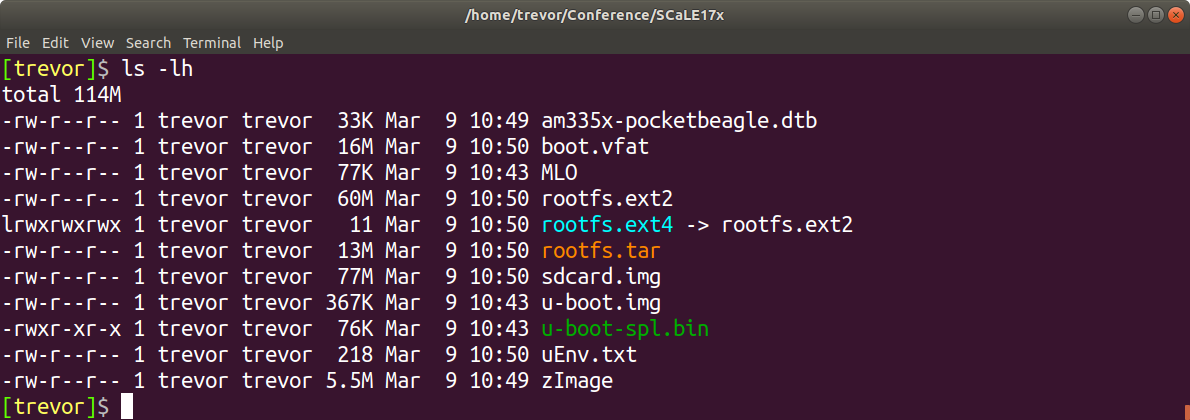
\includegraphics[width=\textwidth]{woerner/buildroot-size.png}

Using {\bf Etcher} or {\bf
dd}, flash this image to your SDcard. Insert the SDcard into your PocketBeagle
and apply power. Ideally you'll have a serial console setup (i.e. {\bf
minicom} or {\bf screen}) so you can watch the progress.

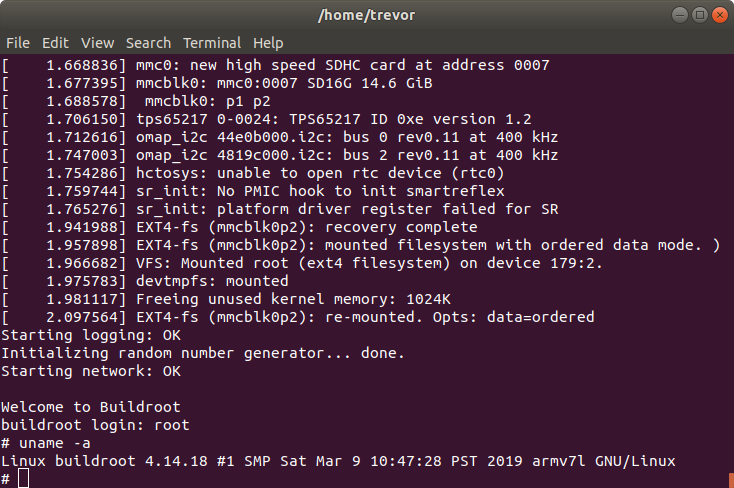
\includegraphics[width=\textwidth]{woerner/buildroot-boot.png}

\end{document}
